\documentclass[../../Report.tex]{subfiles}
\usepackage[italian]{babel}

\begin{document}
\chapter{Valutazione degli Algoritmi di Classificazione}
Nella presente fase del progetto, è stata effettuata la valutazione di tre algoritmi di classificazione: \textbf{KNN}, \textbf{Random Forest} e \textbf{Gaussian Bayes}. L'obiettivo era quello di eseguire un confronto tra i tre algoritmi e di determinare quale di essi fosse più preciso nel classificare i dati utilizzando il dataset HAR fornito.\\
La valutazione è stata effettuata attraverso la misurazione dell'accuratezza degli algoritmi e il confronto dei risultati ottenuti. Questo ha permesso di determinare quale algoritmo fosse il più adatto per il problema di riconoscimento delle attività svolte dall'utente.\\   

\section{Dataset, data mining e tecnologie utilizzate}
Il dataset utilizzato per l'analisi ci è stato fornito dal professor Marco Di Felice. Il dataset è composto da 62.584 osservazioni e 13 colonne riguardanti il valore dei sensori di uno smartphone android e l'attività dell'utente, come seguente:

\begin{table}[H]
    \centering
    \begin{tabular}{|l|p{0.7\linewidth}|}
        \hline
        \textbf{accelerometer\#mean} & la media delle osservazioni dell'accelerometro. \\
        \hline
        \textbf{accelerometer\#min} & l'osservazione minima dell'accelerometro. \\
        \hline
        \textbf{accelerometer\#max} & l'osservazione massima dell'accelerometro. \\
        \hline
        \textbf{accelerometer\#std} & la deviazione standard delle osservazioni dell'accelerometro. \\
        \hline
        \textbf{gyroscope\#mean} & la media delle osservazioni del giroscopio. \\
        \hline
        \textbf{gyroscope\#min} &  l'osservazione minima del giroscopio. \\
        \hline
        \textbf{gyroscope\#max} &  l'osservazione massima del giroscopio. \\
        \hline
        \textbf{gyroscope\#std} & la deviazione standard delle osservazioni del giroscopio. \\
        \hline
        \textbf{gyroscopeuncalibrated\#mean} & la media delle osservazioni del giroscopio non calibrato. \\
        \hline
        \textbf{gyroscopeuncalibrated\#min} &  l'osservazione minima del giroscopio non calibrato. \\
        \hline
        \textbf{gyroscopeuncalibrated\#max} & l'osservazione massima del giroscopio non calibrato. \\
        \hline
        \textbf{gyroscopeuncalibrated\#std} & la deviazione standard delle osservazioni del giroscopio non calibrato.\\
        \hline
        \textbf{target} & l'attività svolta dall'utente. \\
        \hline
    \end{tabular}
\end{table}
Le etichette di questo dataset assumono 5 valori differenti:
\begin{itemize}
    \item \textbf{STILL}: l'utente non si muove.
    \item \textbf{WALKING}: l'utente cammina.
    \item \textbf{CAR}: l'utente è in auto.
    \item \textbf{BUS}: l'utente è in bus.
    \item \textbf{TRAIN}: l'utente è in treno. 
\end{itemize}

\subsection{Data mining}
    Per il data mining è stato utilizzato il linguaggio di programmazione \emph{Python} e per il training e prediction dei modelli la libreria \emph{Scikit-learn}. Inoltre, durante la fase di preprocessing e per la gestione dei dati è stata utilizzata la libreria di Python \emph{Pandas}.\\
    Non è stato fatto un grande preprocessing dei dati, in quanto il dataset fornitoci era già di ottima qualità. Per la rimozione dei valori mancanti, abbiamo rimosso solo le righe per le quali mancavano almeno due attributi per ogni classe di sensori. Questo ci ha portato a perdere circa 5000 tuple. Per quelle righe in cui era presente solamente un valore mancante questo è stato sostituito con la media. I dati sono stati lavorati al fine di eliminare i valori NaN e di normalizzare i dati, scalandoli utilizzando la funzione \emph{MinMaxScaling}. Inoltre sono state eliminate tutte le tuple che non riguardavano le attività di interesse (WALKING e DRIVING).\\
    Per tutti e tre gli algoritmi il dataset è stato suddiviso in due parti:
    \begin{itemize}
        \item \textbf{Training}: è stato utilizzato per il training del modello.
        \item \textbf{Testing}: è stato utilizzato per il testing del modello.
    \end{itemize}
    Per il training è stato utilizzato l'80\% dei dati e per il testing il 20\%.\\

\section{Gli algoritmi}
Come già detto precedentemente, in questa fase di valutazione degli algoritmi di classificazione, sono stati considerati tre differenti approcci: il \textbf{KNN}, il \textbf{Random Forest} e il \textbf{Gaussian Naive Bayes}.\\
Questi algoritmi rappresentano tre approcci distinti alla risoluzione del problema di classificazione, ciascuno con i suoi punti di forza e limiti. Il \textbf{KNN} utilizza una logica basata sulla vicinanza dei dati, il \textbf{Random Forest} è un algoritmo di ensemble che utilizza molteplici alberi di decisione e il \textbf{Gaussian Naive Bayes} si basa sull'assunzione che le feature sono distribuite normalmente.\\
In questa sezione, verranno descritti in dettaglio ciascuno di questi algoritmi e verrà presentato un confronto tra i loro risultati e le loro prestazioni.
\subsection{KNN}
Per quanto riguarda il KNN è stato deciso di effettuare un tuning degli iperparametri per il KNN, con lo scopo di ottenere una prestazione ottimale del modello.\\
I parametri che sono stati modificati sono stati:
\begin{itemize}
    \item \textbf{n\_neighbors}: rappresenta il numero di vicini considerati nella classificazione
    \item \textbf{weights}: determina il peso dei vicini nella classificazione
    \item \textbf{leaf-size}: rappresenta la dimensione massima di una foglia dell'albero di ricerca
    \item \textbf{p}: determina la potenza della metrica utilizzata nella calcoli della distanza tra i vicini
\end{itemize}
Il tuning degli iperparametri è stato effettuato utilizzando la funzione \emph{GridSearchCV} di \emph{Scikit-learn}. Questa funzione permette di eseguire una ricerca su una griglia di valori per gli iperparametri, testando tutte le possibili combinazioni e selezionando quella che produce la migliore prestazione in termini di accuratezza.\\
L'obiettivo di questa ottimizzazione era quello di migliorare la precisione del modello KNN e di fornire una soluzione ottimale per la classificazione dei dati. Il risultato ottenuto ha dimostrato che l'ottimizzazione degli iperparametri è stata efficace e ha contribuito a migliorare la performance del modello.

\subsubsection{Risultati}
I risultati del tuning degli iperparametri utilizzando il dataset precedentemente descritto sono riportati nella tabella seguente:

\begin{table}[H]
    \centering
    \begin{tabular}{|l|c|}
        \hline
         & \textbf{Best value} \\
        \hline
        \textbf{n\_neighbors} & 14 \\
        \hline
        \textbf{weights} & distance \\
        \hline
        \textbf{leaf\_size} & 1 \\
        \hline
        \textbf{p} & 2 \\
        \hline
    \end{tabular}
\end{table}

Con questi parametri siamo riusciti ad ottenere un'accuratezza finale dell'89\%.\\
Facendo training di questo modello con il dataset su cui abbiamo applicato il MinMaxScaling, abbiamo ottenuto un'accuratezza del 90\%.\\
I parametri risultanti dal tuning sono invece:
\begin{table}[H]
    \centering
    \begin{tabular}{|l|c|}
        \hline
         & \textbf{Best value} \\
        \hline
        \textbf{n\_neighbors} & 12 \\
        \hline
        \textbf{weights} & distance \\
        \hline
        \textbf{leaf\_size} & 1 \\
        \hline
        \textbf{p} & 2 \\
        \hline
    \end{tabular}
\end{table}

\begin{figure}[H]
    \centering
    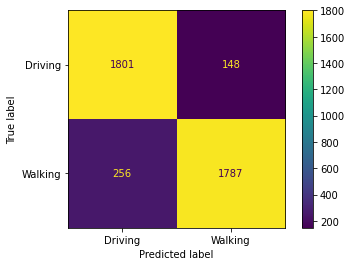
\includegraphics[width=0.49\textwidth]{ConfusionMatrixKNNUnscaled.png}
    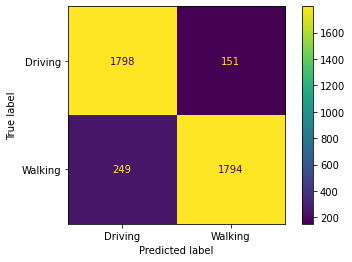
\includegraphics[width=0.49\textwidth]{ConfusionMatrixKNNScaled.png}
    \caption{Matrice di confusione del modello senza scaling (sx) e con scaling (dx)}
    \label{fig:confusion_matrix_KNN}
\end{figure}
Si può notare come questo modello commetta più facilmente errori nel riconoscere la classe DRIVING.\\

\subsection{Random Forest}
Come per il KNN, anche per il Random Forest è stato effettuato un tuning degli iperparametri per ottenere una prestazione ottimale del modello.\
I parametri che sono stati modificati sono stati:
\begin{itemize}
\item \textbf{n\_estimators}: che rappresenta il numero di alberi decisionali nella foresta
\item \textbf{max\_features}: che rappresenta il numero di features da considerare quando si cerca la migliore divisione
\item \textbf{max\_depth}: che rappresenta la profondità massima degli alberi decisionali
\item \textbf{min\_samples\_split}: che rappresenta il numero minimo di campioni richiesti per dividere un nodo interno
\item \textbf{min\_samples\_leaf}: che rappresenta il numero minimo di campioni richiesti per costruire una foglia dell'albero
\item \textbf{bootstrap}: che rappresenta la modalità di campionamento dei dati
\end{itemize}
Il tuning degli iperparametri è stato effettuato utilizzando la funzione \emph{RandomizedSearchCV} di \emph{Scikit-learn}.\\
L'obiettivo di questa ottimizzazione era quello di migliorare la precisione del modello Random Forest e di fornire una soluzione ottimale per la classificazione dei dati. Il risultato ottenuto ha dimostrato che l'ottimizzazione degli iperparametri è stata efficace e ha contribuito a migliorare la performance del modello. La RandomizedSearchCV è stata eseguita per un numero di 100 iterazioni, usando una 5-fold cross validation. Per un totale di 500 fit. In questo caso è stata preferita una RandomizedSearchCV rispetto ad una GridSearchCV poichè il numero di combinazioni di iperparametri da testare è molto elevato e testarli tutti avrebbe richiesto un tempo di esecuzione molto elevato rispetto alla potenza di calcolo disponibile. 

\subsubsection{Risultati}

I risultati del tuning degli iperparametri utilizzando il dataset precedentemente descritto sono riportati nella tabella seguente:

\begin{table}[H]
    \centering
    \begin{tabular}{|l|c|}
        \hline
        & \textbf{Best value} \\
        \hline
        \textbf{n\_estimators} & 800 \\
        \hline
        \textbf{max\_depth} & 90 \\
        \hline
        \textbf{min\_samples\_split} & 5 \\
        \hline
        \textbf{min\_samples\_leaf} & 1 \\
        \hline
        \textbf{max\_features} & sqrt \\
        \hline
        \textbf{bootstrap} & False \\
        \hline
    \end{tabular}
\end{table}

Con questi parametri siamo riusciti ad ottenere un'accuratezza finale del 95.24\% utilizzando il dataset su cui non è stato applicato il MinMaxScaling.

Facendo tuning sul modello Random Forest utilizzando il modello con il MinMaxScaling, si è ottenuto un'accuratezza del 89,95\%.\\
I parametri ottenuti dal tuning sono:

\begin{table}[H]
    \centering
    \begin{tabular}{|l|c|}
        \hline
        & \textbf{Best value} \\
        \hline
        \textbf{n\_estimators} & 1400 \\
        \hline
        \textbf{max\_depth} & 80 \\
        \hline
        \textbf{min\_samples\_split} & 10 \\
        \hline
        \textbf{min\_samples\_leaf} & 2 \\
        \hline
        \textbf{max\_features} & sqrt \\
        \hline
        \textbf{bootstrap} & True \\
        \hline
    \end{tabular}
\end{table}

Mostriamo adesso i grafici delle Matrici di confusione ottenute per i due modelli Random Forest, uno con il dataset su cui non è stato applicato il MinMaxScaling e l'altro con il dataset su cui è stato applicato il MinMaxScaling.

\begin{figure}[H]
    \centering
    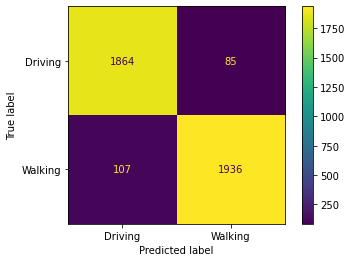
\includegraphics[width=0.49\textwidth]{ConfusionMatrixRFUnscaled.png}
    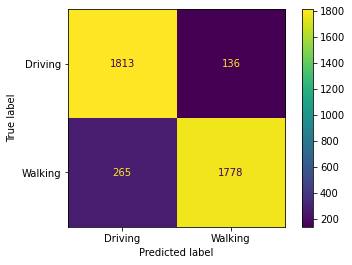
\includegraphics[width=0.49\textwidth]{ConfusionMatrixRFScaled.png}
    \caption{Matrice di confusione del modello senza scaling (sx) e con scaling (dx)}
    \label{fig:confusion_matrix_rf}
\end{figure}
Queste matrici di confusione mostrano come il modello Radom Forest sia ottimo per la classificazione di questo tipo dati. Sia il modello senza scaling che quello con scaling sono in grado di classificare correttamente la maggior parte dei dati, ma è possibile notare cme riescano a riconoscere più facilmente l'etichetta WALKING, rispetto a quella DRIVING, nella quale è presente un errore maggiore. 
\subsection{Gaussian Naive Bayes}
Per quanto riguarda il Gaussian Naive Bayes, abbiamo deciso di utilizzare questo algoritmo per la classificazione dei dati in quanto si tratta di un metodo semplice e veloce per la classificazione basato sull'assunzione che le feature siano distribuite secondo una distribuzione normale.\\
In questo caso, non era necessario effettuare un tuning degli iperparametri, in quanto il Gaussian Naive Bayes non ha parametri che possono essere ottimizzati per migliorare le sue prestazioni.

\subsubsection{Risultati}
Il modello Gaussian Naive Bayes ha fornito un'accuratezza del 81.82\%, che risulta essere un risultato inferiore rispetto ai modelli KNN e Random Forest.

\section{Confronto dei risultati}
Illustriamo di seguito i risultati completi dei tre modelli precedenti, ottenute utilizzando il dataset precedentemente descritto.

\begin{table}[H]
    \begin{center}
        \begin{tabular}{ |P{2cm}|P{1cm}|P{1cm}|P{1cm}|P{1cm}|P{1cm}|P{1cm}|P{1cm}|P{1cm}|P{1cm}|P{1.8cm}| } 
            \multicolumn{11}{c}{\textbf{Evaluating algorithms}} \\
            \hline
            & \multicolumn{3}{c|}{\textbf{KNN}} & \multicolumn{3}{c|}{\textbf{RF}} & \multicolumn{3}{c|}{\textbf{GNB}} & \\
            \hline
            \rowcolor{lightgray}
            & \textbf{P} & \textbf{R} & \textbf{F1} & \textbf{P} & \textbf{R} & \textbf{F1} & \textbf{P} & \textbf{R} & \textbf{F1} & \textbf{Support} \\
            \hline
            \textbf{0} & 0.88 & 0.92 & 0.90 & 0.95 & 0.95 & 0.95 & 0.76 & 0.98 & 0.86 & 1949 \\
            \hline
            \rowcolor{lightgray}
            \textbf{1} & 0.92 & 0.87 & 0.90 & 0.95 & 0.95 & 0.95 & 0.98 & 0.71 & 0.82 & 2043 \\
            \hline
            \textbf{Accuracy} & \multicolumn{3}{c|}{0.8987975951903807} &\multicolumn{3}{c|}{0.9524048096192385} &\multicolumn{3}{c|}{0.843436873747495}& 3992 \\
            \hline
            \rowcolor{lightgray}
            \textbf{Macro AVG} & 0.90 & 0.90 & 0.90 &0.95  & 0.95 & 0.95 & 0.87 & 0.85 & 0.84 & 3992 \\
            \hline
            \textbf{Weighted AVG} & 0.90 & 0.90 & 0.90 & 0.95 & 0.95 & 0.95 & 0.87 & 0.84 & 0.84 & 3992 \\
            \hline
        \end{tabular}
        \caption{P = Precision, R = Recall e F1 = F1-score}
    \end{center}
\end{table}

Utilizzando il dataset su cui è stato applicato il MinMaxScaling i risultati sono:
\begin{table}[H]
    \begin{center}
        \begin{tabular}{ |P{2cm}|P{1cm}|P{1cm}|P{1cm}|P{1cm}|P{1cm}|P{1cm}|P{1cm}|P{1cm}|P{1cm}|P{1.8cm}| } 
            \multicolumn{11}{c}{\textbf{Evaluating algorithms}} \\
            \hline
            & \multicolumn{3}{c|}{\textbf{KNN}} & \multicolumn{3}{c|}{\textbf{RF}} & \multicolumn{3}{c|}{\textbf{GNB}} & \\
            \hline
            \rowcolor{lightgray}
            & \textbf{P} & \textbf{R} & \textbf{F1} & \textbf{P} & \textbf{R} & \textbf{F1} & \textbf{P} & \textbf{R} & \textbf{F1} & \textbf{Support} \\
            \hline
            \textbf{0} & 0.88 & 0.88 & 0.92 & 0.87 & 0.93 & 0.90 & 0.76 & 0.98 & 0.86 & 1949 \\
            \hline
            \rowcolor{lightgray}
            \textbf{1} & 0.92 & 0.88 & 0.90 & 0.93 & 0.87 & 0.90 & 0.98 & 0.71 & 0.82 & 2043 \\
            \hline
            \textbf{Accuracy} & \multicolumn{3}{c|}{0.8997995991983968} &\multicolumn{3}{c|}{0.8995490981963928} &\multicolumn{3}{c|}{0.843436873747495}& 3992 \\
            \hline
            \rowcolor{lightgray}
            \textbf{Macro AVG} & 0.90 & 0.90 & 0.90 &0.90  & 0.90 & 0.90 & 0.87 & 0.85 & 0.84 & 3992 \\
            \hline
            \textbf{Weighted AVG} & 0.90 & 0.90 & 0.90 & 0.90 & 0.90 &0.90  & 0.87 & 0.84 & 0.84 & 3992 \\
            \hline

        \end{tabular}
        \caption{P = Precision, R = Recall e F1 = F1-score}
    \end{center}
\end{table}



\end{document}